\section{Narzędzia rysowania i edycji}
\label{sec:narzedzia_rysowania_i_edycji}

W celu umożliwienia użytkownikowi projektowania schematów układów scalo\-nych,
w grze zaimplementowano zestaw narzędzi do rysowania i edycji, których założenia przedstawiono w podrozdziale~\ref{sec:zalozenia_funkcjonalne}.
Podobnie jak w przypadku warstw, narzędzia są wstępnie definiowane w pliku konfiguracyjnym SO, \texttt{ToolConfig}.
Zawiera on informacje o wskazówce dla narzędzia, ikonie, przypisanym skrócie klawiszowym, czy jest używane do edytowania zaznaczenia
oraz o grafice i hotspocie niestandardowego kursora.
Przykładową konfigurację przedstawiono na rys.~\ref{fig:tool_config}.

\begin{figure}[h!]
    \centering
    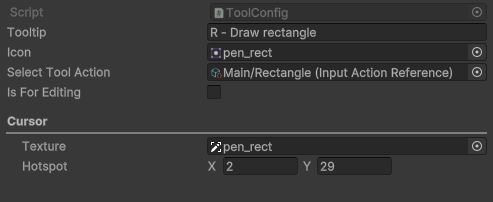
\includegraphics[width=0.9\textwidth]{chapters/chapter4/rys/tool_config}
    \caption[Przykładowa konfiguracja narzędzia.]{Przykładowa konfiguracja narzędzia, źródło: opracowanie własne.}
    \label{fig:tool_config}
\end{figure}

Narzędziami zarządza \texttt{ToolsManager}, odpowiadający za wybór aktywnego narzędzia,
a także zmianę ikony kursora w zależności od wybranego narzędzia.
Implementuje on także klasę \texttt{MonoSingleton}, aby ułatwić dostęp do niego z innych komponentów.
Ze względu na większą autonomię narzędzi w porównaniu do warstw,
dla każdego z nich stworzono osobny obiekt na scenie, z którym związane są wszystkie operacje rysowania lub edycji.
Wspólnym rodzicem narzędzi jest obiekt \texttt{Tools}, na którym znajduje się \texttt{ToolsManager},
rys.~\ref{fig:tools_hierarchy}.

\begin{figure}[h!]
    \centering
    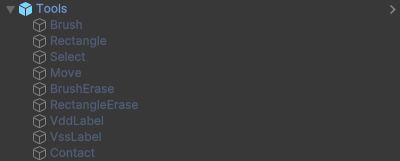
\includegraphics[width=0.9\textwidth]{chapters/chapter4/rys/tools_hierarchy}
    \caption[Hierarchia obiektów narzędzi na scenie.]{Hierarchia obiektów narzędzi na scenie, źródło: opracowanie własne.}
    \label{fig:tools_hierarchy}
\end{figure}

%\begin{figure}[h]
%    \centering
%    \begin{subfigure}{.45\textwidth}
%        \centering
%        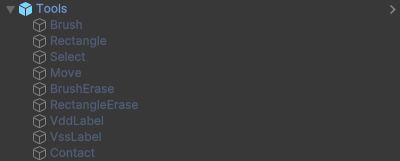
\includegraphics[width=.5\linewidth]{chapters/chapter4/rys/tools_hierarchy}
%        \caption{Hierarchia obiektów narzędzi na scenie.}
%        \label{fig:tools_hierarchy}
%    \end{subfigure}
%    \begin{subfigure}{.45\textwidth}
%        \centering
%        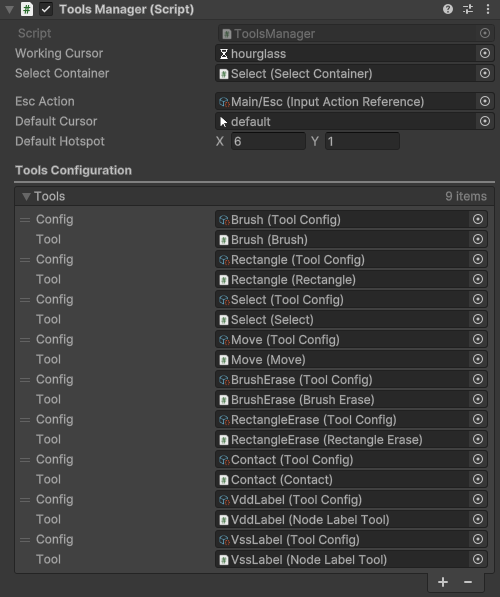
\includegraphics[width=.5\linewidth]{chapters/chapter4/rys/tools_manager}
%        \caption{Widok inspektora menedżera narzędzi.}
%        \label{fig:tools_manager}
%    \end{subfigure}
%    \caption[Widok narzędzi na scenie oraz inspektora komponenetu zarządzającego nimi.]
%    {
%        Widok narzędzi na scenie oraz inspektora komponenetu zarządzającego nimi,
%        źródło: opracowanie własne.
%    }
%    \label{fig:tools}
%\end{figure}

%\newpage % TODO: check this if something changes

Ponieważ narzędzia są od początku obecne na scenie, 
do \texttt{ToolsManager} należało przypisać referencje do konfiguracji narzędzi wraz z samymi obiektami narzędzi,
jak pokazano na rys.~\ref{fig:tools_manager}.
W tym celu przygotowano dodatkowo strukturę \texttt{ToolHolder},
która przechowuje obie referencje.
W przypadku narzędzia potrzebne było jeszcze,
aby dziedziczyło ono po klasie \texttt{ToolAbstaract}.
%Dzięki czemu można przekazać, a później także zarządzać narzędziami niezależnie od ich funkcji. 
%Dzięki czemu również można było zarządzać narzędziami niezależnie od ich funkcji.
Dzięki temu można zarządzać narzędziami niezależnie od ich funkcji.

\begin{figure}[h!]
    \centering
    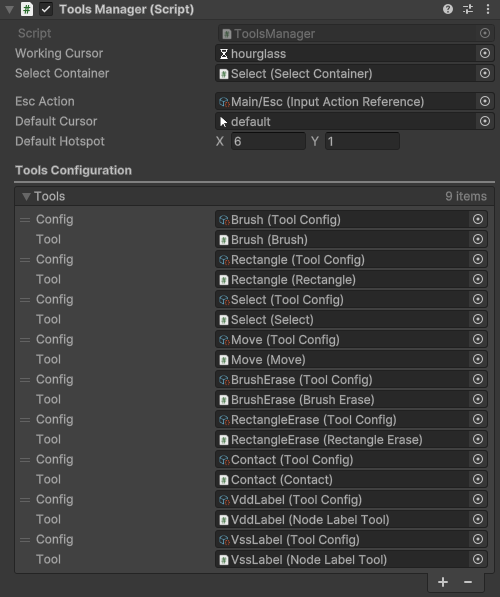
\includegraphics[width=0.9\textwidth]{chapters/chapter4/rys/tools_manager}
    \caption[Widok inspektora menedżera narzędzi.]{Widok inspektora menedżera narzędzi, źródło: opracowanie własne.}
    \label{fig:tools_manager}
\end{figure}

Wśród narzędzi można wyróżnić dwa główne typy różniące się pod kątem sposobu działania, punktowe i obszarowe.
Ze względu na ten podział korzystają one również z innych funkcji w celu wykrywania komórek.
Narzędzia punktowe działają jedynie na jedną komórkę jednocześnie,
z tego powodu do wykrywania komórek używają funkcji \texttt{Physics.Raycast}.
Sprawdza ona, czy w prostej linii występuje kolizja z obiektem posiadającym komponent \texttt{Collider}.\\
\indent W przypadku narzędzi obszarowych wykrywanie odbywa się poprzez rozciąganie detektora w narzędziu,
którym jest \texttt{BoxCollider} z zaznaczoną opcją \textit{Is Trigger}.
%, przedstawioną na listingu~\ref{lst:drag_update}.
Istotne jest także,
aby detektor zawsze był minimalnie mniejszy od wymiaru obszaru w celu uniknięcia wykrycia komórek jedynie sąsiadujących z nim.
%\begin{lstlisting}[language={C},label=lst:drag_update,caption={Metoda \texttt{DragUpdate} używana w narzędziach obszarowych}]
private void ModifyBounds(float deltaX, float deltaY) {
    detector.size = new Vector3(deltaX-0.1f, deltaY-0.1f, 0.1f);
    detector.center = new Vector3(deltaX / 2, deltaY / 2, 0);
    layerSprite.size = new Vector2(deltaX, deltaY);
}
\end{lstlisting}
W momencie kolizji detektora z komórką w narzędziu wywoływana jest funkcja \texttt{OnTriggerEnter},
która zwraca referencję do komórki, z którą nastąpiła kolizja.
Po wyjściu z kolizji wywoływana jest funkcja \texttt{OnTriggerExit}.
Dzięki wykorzystaniu tych funkcji możliwe jest wykrywanie komórek w trakcie pracy narzędzia,
przez co nie ma potrzeby znajdywania ich wszystkich w jednym kroku.
Prócz komponentu \texttt{BoxCollider} narzędzia obszarowe posiadają także komponent \texttt{SpriteRenderer},
dzięki któremu można wyświetlać zarys pola, które jest aktualnie rysowane.
Za modyfikowanie sprite'a, \texttt{BoxCollider}'a oraz obliczanie wymiarów obszaru odpowiada metoda \texttt{OnDragUpdate}. 
%Wspólna dla wszystkich obszarowych narzędzi jest także metoda \texttt{OnDragUpdate},% przedstawiona na listingu~\ref{lst:drag_update},
%która przy aktywnym narzędziu, co klatkę aktualizuje obszar,
%przy okazji rozciągając sprite dający możliwość pokazania jego zarysu.
%W funkcji tej jest wywoływana także metoda \texttt{ModifyBounds}.
Kolejną wspólną cechą dla tego typu są dwa tryby działania,
w jednym z nich prostokątne pole jest tworzone poprzez przeciągnięcie kursora,
natomiast w drugim poprzez kliknięcie w dwa punkty,
przy jednocześnie wciśniętym klawiszu modyfikatora~\textt{Shift}, co tworzy obszar między nimi.

\subsection{Pędzel}
\label{subsec:pedzel}

Pędzel jest narzędziem punktowym, służącym do precyzyjniejszego rysowania pojedynczych komórek.
Charakteryzuje się działaniem ciągłym, dopóki lewy przycisk myszy jest wciśnięty.
W przypadku tego narzędzia potrzebne było wykrywanie komórek jedynie tej warstwy, która jest obecnie wybrana,
stąd promień w funkcji \texttt{Physics.Raycast} musi zaczynać się tuż nad tą warstwą
i być na tyle krótki, by nie wykrywać komórek z innych warstw.
Ponieważ czas pomiędzy kolejnymi klatkami jest większy niż czas odświeżania myszy,
potrzebne jest dodatkowe sprawdzenie, czy przesunięcie względem poprzedniej pozycji nie jest za duże,
w przypadku gdy miało to miejsce, należało wypełnić obszar między dwoma punktami.
Służy do tego funkcja \texttt{DrawInterpolate},
rysująca linię między obecnym a poprzednim punktem.
Skonfigurowany pędzel przedstawiono na rys.~\ref{fig:brush}.

\begin{figure}[h!]
    \centering
    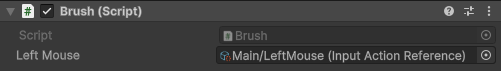
\includegraphics[width=0.9\textwidth]{chapters/chapter4/rys/tools/brush}
    \caption[Skonfigurowane narzędzie pędzla.]{Skonfigurowane naarzędzie pędzla, źródło: opracowanie własne.}
    \label{fig:brush}
\end{figure}
%, przedstawiona na listingu~\ref{lst:draw_interpolate}.
%\begin{lstlisting}[language={C},label=lst:draw_interpolate,caption={Metoda \texttt{DrawInterpolate} interpolująca pomiędzy dwoma punktami}]
private void DrawInterpolate(float dX, float dY) {
    var axis = dX > dY ? 1 : 0; // 1 - horizontal axis, 0 - vertical axis
    var dirX = _gridPos.x > _oldGridPos.x ? 1 : -1;
    var dirY = _gridPos.y > _oldGridPos.y ? 1 : -1;
    if ((int)dX == 0 || (int)dY == 0) {
        StraightLine((int)dX, (int)dY);
        return;
    }
    var step = dX > dY ? dX / dY : dY / dX;
    float rest = 0f;
    float sum = 0f;
    var bigger = dX > dY ? dX : dY;
    var curX = _oldGridPos.x;
    var curY = _oldGridPos.y;
    while (sum < bigger) {
        rest += step;
        var amount = (int)Mathf.Floor(rest);
        rest -= amount;
        if (axis == 1) // horizontal {
            DrawForHorizontal(amount, dirX, curX, curY);
            curY += dirY;
        }
        else // vertical {
            DrawForVertical(amount, dirY, curX, curY);
            curX += dirX;
        }
        sum += step;
    }
    Draw(_gridPos.x, _gridPos.y); // make sure to draw the last pixel  
}
\end{lstlisting}

\subsection{Rysowanie prostokątne}
\label{subsec:rysowanie_prostokatne}

Narzędzie rysowania prostokątnego jest narzędziem obszarowym.
Podobnie jak w przypadku pędzla detekcja komórek odbywa się jedynie na poziomie jednej warstwy,
po zakończeniu zaznaczania sprawdzana jest po kolei każda pozycja z obszaru czy nie pokrywa się z którąś z komórek,
gdy pozycja jest niezajęta, narysowana może zostać nowa komórka.
Widok inspektora narzędzia przedstawiono na rys.~\ref{fig:rectangle}.

\begin{figure}[h!]
    \centering
    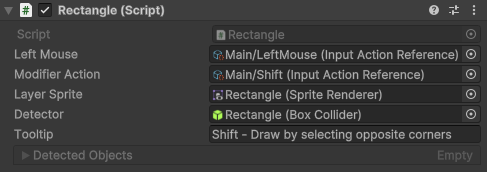
\includegraphics[width=0.9\textwidth]{chapters/chapter4/rys/tools/rectangle}
    \caption[Skonfigurowane narzędzie rysowania prostokątnego.]{Skonfigurowane narzędzie rysowania prostokątnego, źródło: opracowanie własne.}
    \label{fig:rectangle}
\end{figure}

\subsection{Gumka i usuwanie obszarowe}
\label{subsec:gumka_i_usuwanie_obszarowe}

Gumka i usuwanie prostokątnego obszaru działają na podobnej zasadzie jak odpowiednio pędzel
i narzędzie rysowania prostokątnego, przy czym mają na celu usuwanie komórek.
Główną różnicą jest to, że długość promienia w funkcji \texttt{Physics.Raycast} dla gumki jest większa,
co pozwala na wykrycie po kolei wszystkich komórek dla każdej z warstw.
Podobnie w przypadku usuwania obszarowego,
\textt{BoxCollider} będący detektorem musi być większy w osi Z tak, aby mógł nachodzić na komórki ze wszystkich warstw.
Widok inspektora narzędzia gumki przedstawiono na rys.~\ref{fig:erase},
a narzędzia usuwania obszarowego na rys.~\ref{fig:recta_erase}.

\begin{figure}[h!]
    \centering
    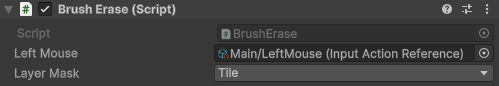
\includegraphics[width=0.9\textwidth]{chapters/chapter4/rys/tools/brush_erase}
    \caption[Skonfigurowane narzędzie gumki.]{Skonfigurowane narzędzie gumki, źródło: opracowanie własne.}
    \label{fig:erase}
\end{figure}

\begin{figure}[h!]
    \centering
    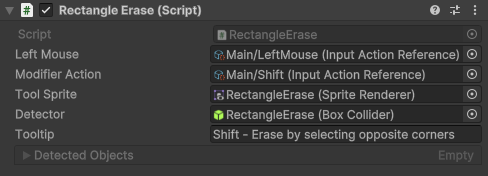
\includegraphics[width=0.9\textwidth]{chapters/chapter4/rys/tools/rectangle_erase}
    \caption[Skonfigurowane narzędzie usuwania obszarowego.]
    {Skonfigurowane narzędzie usuwania obszarowego, źródło: opracowanie własne.}
    \label{fig:recta_erase}
\end{figure}

\subsection{Zaznaczanie}
\label{subsec:zaznaczanie}

Zaznaczanie jest narzędziem obszarowym, pozwalającym na wybranie komórek w celu ich edycji.
Podobnie jak w przypadku usuwania obszarowego,
\textt{BoxCollider} musi być większy,
aby mógł wykrywać komórki ze wszystkich warstw.
Po zakończeniu zaznaczania,
referencje do wykrytych obiektów są przekazywane do oddzielnego komponentu \texttt{SelectContainer}
i zapisywane w liście.
Następnie zwiększa się w nich przezroczystość oraz zmienia się warstwę w Unity na \textit{Selection},
co pozwala na ich wyróżnienie oraz lepszą filtrację.
Dzięki wykorzystaniu osobnego komponentu można niezależnie,
względem samego narzędzia,
kontrolować zaznaczone komórki.
W przypadku trybu dodawania zaznaczenia proces jest identyczny, jak przy samym zaznaczaniu,
natomiast w trybie odejmowania,
wykryte obiekty są usuwane z listy w \texttt{SelectContainer}, a ich kolor i warstwa Unity resetowane.
Ponowne zaznaczenie komórek bez dodatkowego trybu resetuje zaznaczenie,
podobnie jak wybranie innego narzędzia nieoznaczonego jako do edycji bądź wciśnięcie klawisza~\textt{Esc}.
Skonfigurowane narzędzie zaznaczania przedstawiono na rys.~\ref{fig:select}.

\begin{figure}[h!]
    \centering
    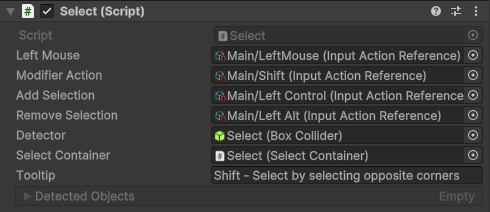
\includegraphics[width=0.9\textwidth]{chapters/chapter4/rys/tools/select}
    \caption[Skonfigurowane narzędzie zaznaczania.]{Skonfigurowane narzędzie zaznaczania, źródło: opracowanie własne.}
    \label{fig:select}
\end{figure}

\subsection{Przesuwanie}
\label{subsec:przesuwanie}

Przesuwanie jako jedyne nie należy do żadnego z wcześniej wymienionych typów,
gdyż jest narzędziem edycji zaznaczenia.
Przesunąć zaznaczony obszar można poprzez przeciągnięcie go w dowolnym kierunku.
Przy każdym kliknięciu przycisku myszy uprzednio sprawdzane jest,
czy \texttt{SelectContainer} posiada zaznaczenie,
%i czy kliknięto miejsce, gdzie ono występuje,
do tego weryfikowane jest, czy kliknięto miejsce, gdzie ono występuje.
W tym celu ponownie wykorzystano \texttt{Physics.Raycast} z tą różnicą,
że dodano filtracje po warstwach Unity, aby wykryć jedynie obiekty należące do warstwy \textit{Selection}.
W przypadku gdy zaznaczenie jest wykryte, \texttt{SelectContainer} ustawia jako rodzica zaznaczonych obiektów,
obecne narzędzie.
Ponieważ w Unity pozycja rodzica kontroluje również pozycję dzieci,
można dzięki temu przesuwać zaznaczone obiekty wraz z narzędziem.
Samo przesuwanie odbywa się poprzez nadpisanie pozycji kursora w przestrzeni roboczej, na pozycję narzędzia.
%jak pokazano na listingu~\ref{lst:movement_update}.
%Po puszczeniu przycisku myszy i zakończeniu przesuwania, zaznaczone obiekty są zwracane do oryginalnych rodziców,
%poprzez odpowiednie posortowanie komórek po ich tagach, czymzajmuje się komponent \texttt{SelectContainer}.
%\begin{lstlisting}[language={C},label=lst:movement_update,caption={Metoda \texttt{MovementUpdate} aktualizująca pozycję narzędzia przesuwania}]
private void MovementUpdate() {
    var gridPosition = MouseGrid.GridPos;
    var position = transform.position;
    position.x = gridPosition.x;
    position.y = gridPosition.y;
    transform.position = position;
    SizeX = (int) (gridPosition.x - _dragOrigin.x);
    SizeY = (int) (gridPosition.y - _dragOrigin.y);
}
\end{lstlisting}
Po zakończeniu przesuwania i puszczeniu przycisku myszy,
zaznaczone obiekty są zwracane do swoich oryginalnych rodziców.
Proces ten polega na odpowiednim posortowaniu komórek według ich tagów, 
odpowiada za to komponent \texttt{SelectContainer}.
Widok skonfigurowanego narzędzia przesuwania przedstawiono na rys.~\ref{fig:move}.

\begin{figure}[h!]
    \centering
    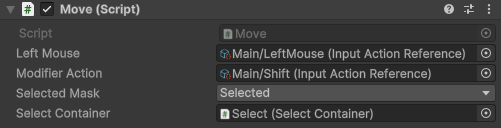
\includegraphics[width=0.9\textwidth]{chapters/chapter4/rys/tools/move}
    \caption[Skonfigurowane narzędzie przesuwania.]{Skonfigurowane narzędzie przesuwania, źródło: opracowanie własne.}
    \label{fig:move}
\end{figure}

\subsection{Kontakty między warstwami}
\label{subsec:kontakty}

Rysowanie kontaktów działa podobnie jak w przypadku rysowania prostokątnego,
natomiast zamiast wielu komórek rysowana jest tylko jedna na cały obszar.
%Podobnie do zaznaczania, czy usuwania obszarowego detektor jest większy,
%aby wykryć, z jakimi warstwami przecina się kontakt.
%W przypadku gdy wykryto inną ilość warstw niż dwie lub inny kontakt, kontakt nie jest rysowany.
Podobnie jak przy zaznaczaniu lub usuwaniu obszarowym,
detektor został zwiększony, aby wykryć,
z którymi warstwami przecina się kontakt.
Jeśli wykryta liczba warstw różni się od dwóch lub zostanie wykryty inny kontakt,
rysowanie zostaje przerwane.
Widok narzędzia rysowania kontaktów przedstawiono na rys.~\ref{fig:contact}.

\begin{figure}[h!]
    \centering
    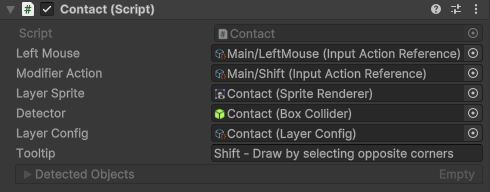
\includegraphics[width=0.9\textwidth]{chapters/chapter4/rys/tools/contact}
    \caption[Skonfigurowane narzędzie rysowania kontaktów.]
        {Skonfigurowane narzędzie rysowania kontaktów, źródło: opracowanie własne.}
    \label{fig:contact}
\end{figure}

\subsection{Oznaczenia zasilania ($V_{DD}$) i masy ($V_{SS}$)}
\label{subsec:oznaczenia_zasilania}

%Oznaczenia są również rysowane jako komórki.
%Każda z nich zawiera dodatkowo komponent \texttt{NodeLabel},
%w którym przy tworzeniu oznaczenia przypisywany jest odpowiedni typ, $V_{DD}$ lub $V_{SS}$.
%Do narysowania obu oznaczeń służy ten sam komponent \texttt{NodeLabelTool},
%natomiast w różnych konfiguracjach, dzięki czemu do obu oznaczeń są dwa osobne narzędzia.
%Aby wyegzekwować oznaczanie tylko na warstwach metalu,
%przy użyciu \texttt(Physics.Raycast),
%sprawdzane jest czy pod wybraną pozycją znajduje się komórka z warstwy metalu,
%poprzez zweryfikowanie tagu obiektu, jaki został wykryty, czy jest równy \textit{Metal 1} lub \textit{Metal 2}.
%Ponieważ może być tylko jedno oznaczenie danego typu na schemacie,
%\texttt{NodeLabelTool} przy tworzeniu nowej komórki zapisuje referencję do niej.
%Gdy ponownie jest używane narzędzie, zmieniana jest jedynie pozycja istniejącego oznaczenia.
Oznaczenia są rysowane jako komórki,
z których każda zawiera komponent \texttt{NodeLabel}.
Podczas tworzenia oznaczenia przypisywany jest mu odpowiedni typ: $V_{DD}$ lub $V_{SS}$.
Do rysowania obu typów oznaczeń wykorzystuje się komponent \texttt{NodeLabelTool},
co pozwala na stworzenie dwóch oddzielnych narzędzi dla każdego oznaczenia,
ale jednoczesne wykorzystanie tych samych komponentów.
Aby umożliwić oznaczanie wyłącznie na warstwach metalu, narzędzie wykorzystuje \texttt{Physics.Raycast},
aby sprawdzić, czy pod wybraną pozycją znajduje się komórka z warstwy metalu.
Weryfikacja odbywa się poprzez sprawdzenie tagu obiektu, czy jest równy \textit{Metal 1} lub \textit{Metal 2}.
Ponieważ na schemacie może znajdować się tylko jedno oznaczenie danego typu,
\texttt{NodeLabelTool} przechowuje referencję do już istniejącej komórki.
Przy ponownym użyciu narzędzia zmieniana jest jedynie pozycja istniejącego oznaczenia.
Widok inspektora narzędzia oznaczeń przedstawiono na rys.~\ref{fig:label}.

\begin{figure}[h!]
    \centering
    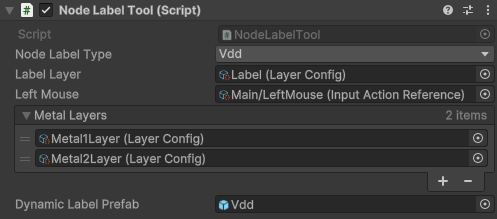
\includegraphics[width=0.9\textwidth]{chapters/chapter4/rys/tools/node_label_tool}
    \caption[Skonfigurowane narzędzie oznaczeń dla typu $V_{DD}$.]
    {Skonfigurowane narzędzie oznaczeń dla typu $V_{DD}$, źródło: opracowanie własne.}
    \label{fig:label}
\end{figure}


